\documentclass[aspectratio=169]{beamer}
\setbeamertemplate{navigation symbols}{}
\usepackage{color,amsmath,comment, subfigure}
\usepackage{booktabs}
\usepackage{url}


%%%%%%%%%%%%%%%%%%%%%%%%%%
\title[]{Class 13: Respondent-driven sampling}
\author[]{Matthew J. Salganik}
\institute[]{Sociology 204: Social Networks\\Princeton University}
\date[]{
3/3 New approaches to respondent-driven sampling
\vfill
\begin{flushleft}
\vspace{0.6in}

\includegraphics[width=0.1\textwidth]{figures/cc.png}
\end{flushleft}

}

\begin{document}
%%%%%%%%%%%%%%%%%%%%%%%%%%%
\frame{\titlepage}
%%%%%%%%%%%%%%%%%%%%%%%%%%%
\begin{frame}

In the previous video we saw that even if assumptions are met, respondent-driven sampling seems to have high sample-to-sample variability in real social networks.  Could we improve respondent-driven sampling to address these problems?

3 approaches:
\begin{itemize}
\item change offspring distribution
\item change data collection to avoid bottlenecks
\item diagnostics to detect problems
\end{itemize}

\end{frame}
%%%%%%%%%%%%%%%%%%%%%%%%%%%%%%%%%
\frame{
\frametitle{How can we improve RDS?}

Change offspring distribution by changing from 3 to 2 coupons. Switching from:
\begin{center}
{\tiny
\begin{tabular}{lcccc}
\toprule
& \multicolumn{4}{c}{Number of recruits}\\
\cmidrule{2-5}
 & 0 & 1 & 2 & 3 \\ 
\midrule
Prob. & 1/3 & 1/6 & 1/6 & 1/3\\
\bottomrule
\end{tabular}
}
\end{center}
\begin{center}to\end{center}
\begin{center}
\tiny{
\begin{tabular}{lccc}
\toprule
& \multicolumn{3}{c}{Number of recruits}\\
\cmidrule{2-4}
 & 0 & 1 & 2 \\ 
\midrule
Prob. & 1/4 & 1/4 & 1/2\\
\bottomrule
\end{tabular}
}
\end{center}
reduces design effects for prop. female and prop. non-white by about 20\% in Add Health data.
}
%%%%%%%%%%%%%%%%%%%%%%%%%%%%%%%
\frame{
\frametitle{Reducing multiple recruitment improves estimates}
\begin{figure}
  \centering
     \subfigure[Prop. non-White]{
     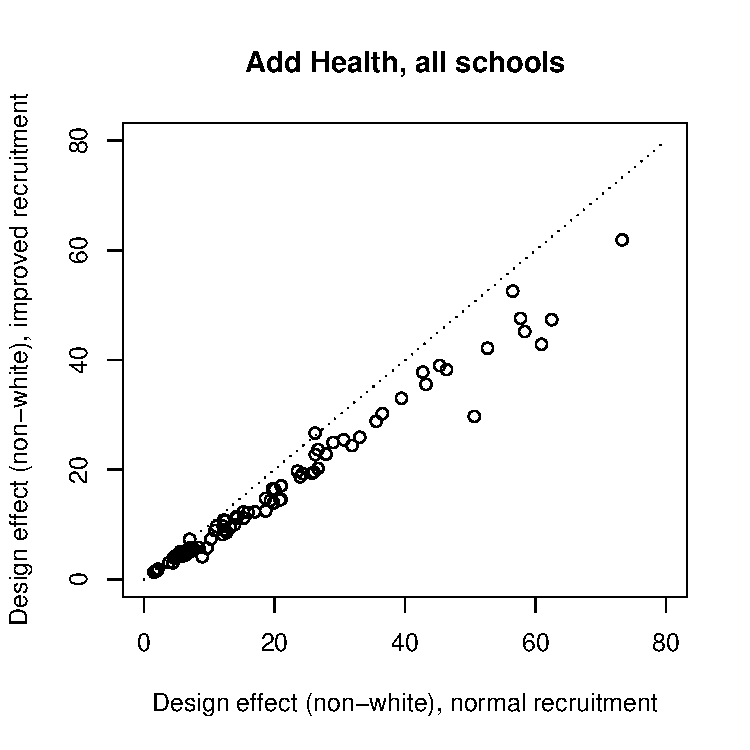
\includegraphics[width=0.45\textwidth]{figures/addhealth_de_nonwhite_normalrec_improvedrec}}
  \hspace{0in}
    \subfigure[Prop. Female]{
    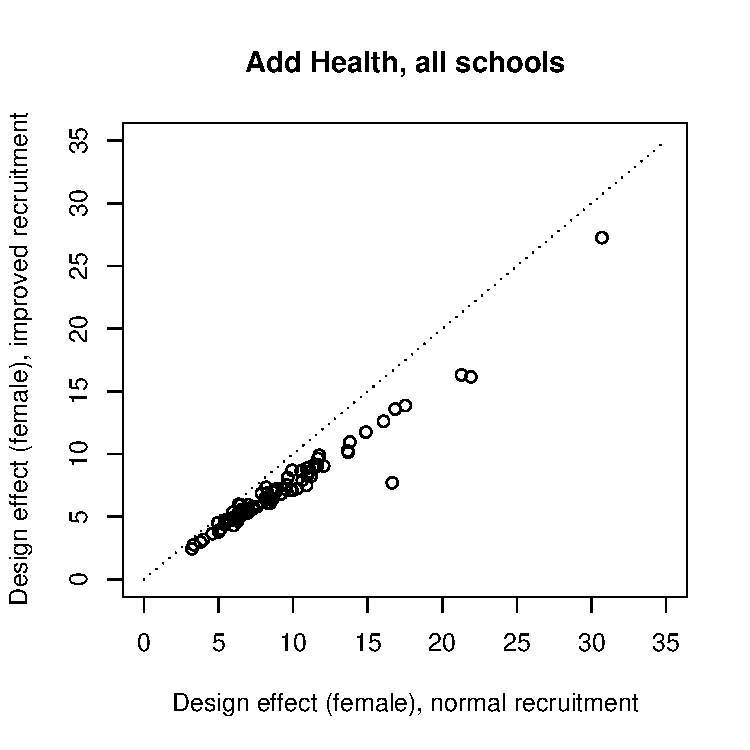
\includegraphics[width=0.45\textwidth]{figures/addhealth_de_female_normalrec_improvedrec}}
\end{figure}
}
%%%%%%%%%%%%%%%%%%%%%%%%%%%%%%%
\begin{frame}

New approaches to sample that avoid bottlenecks. 

\end{frame}
%%%%%%%%%%%%%%%%%%%%%%%%%%%%%%%%%
\begin{frame}

\begin{center}
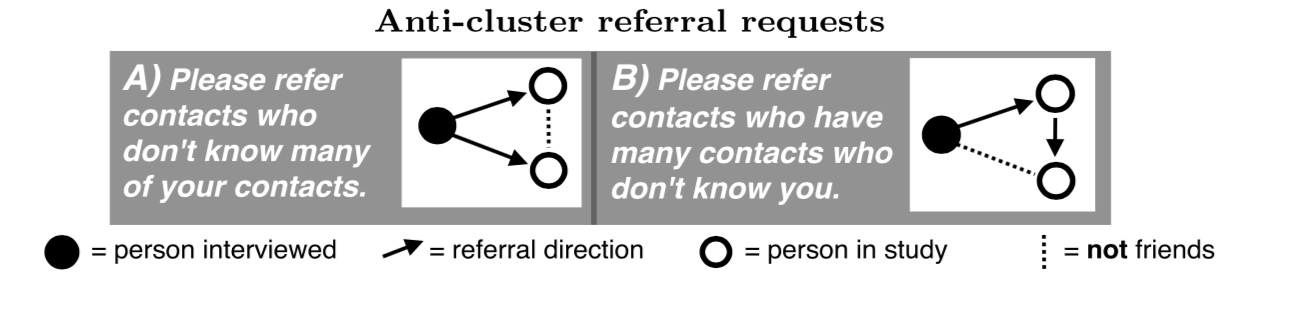
\includegraphics[width=0.8\textwidth]{figures/khabbazian_novel_2017_fig1}
\end{center}


\end{frame}
%%%%%%%%%%%%%%%%%%%%%%%%%%%%%%%%%
\begin{frame}

\begin{center}
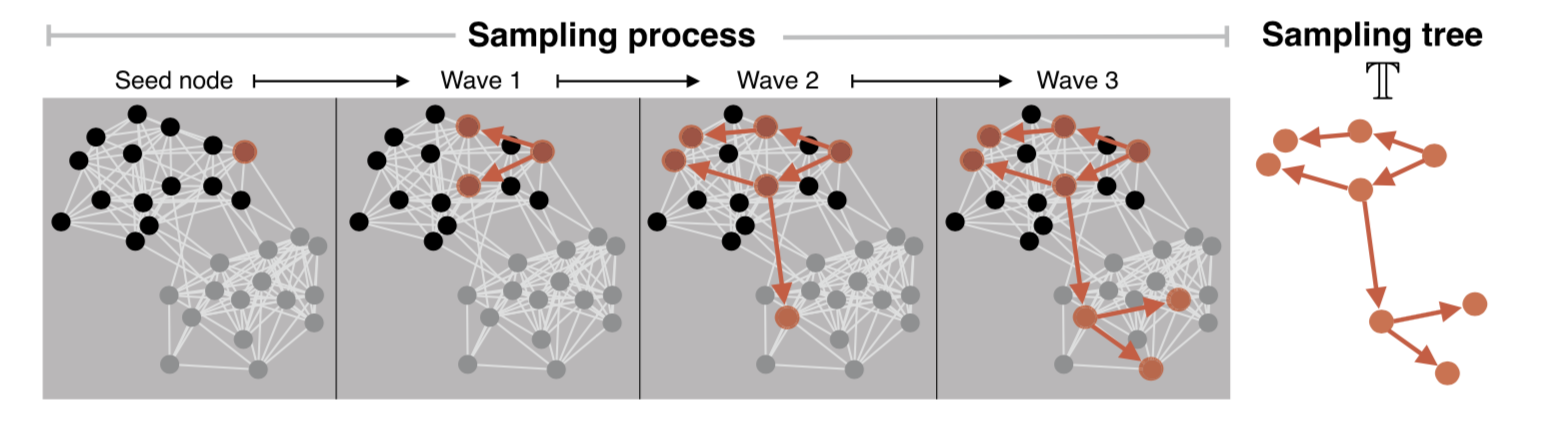
\includegraphics[width=0.8\textwidth]{figures/khabbazian_novel_2017_fig2}
\end{center}

\end{frame}
%%%%%%%%%%%%%%%%%%%%%%%%%%
\begin{frame}

\begin{center}
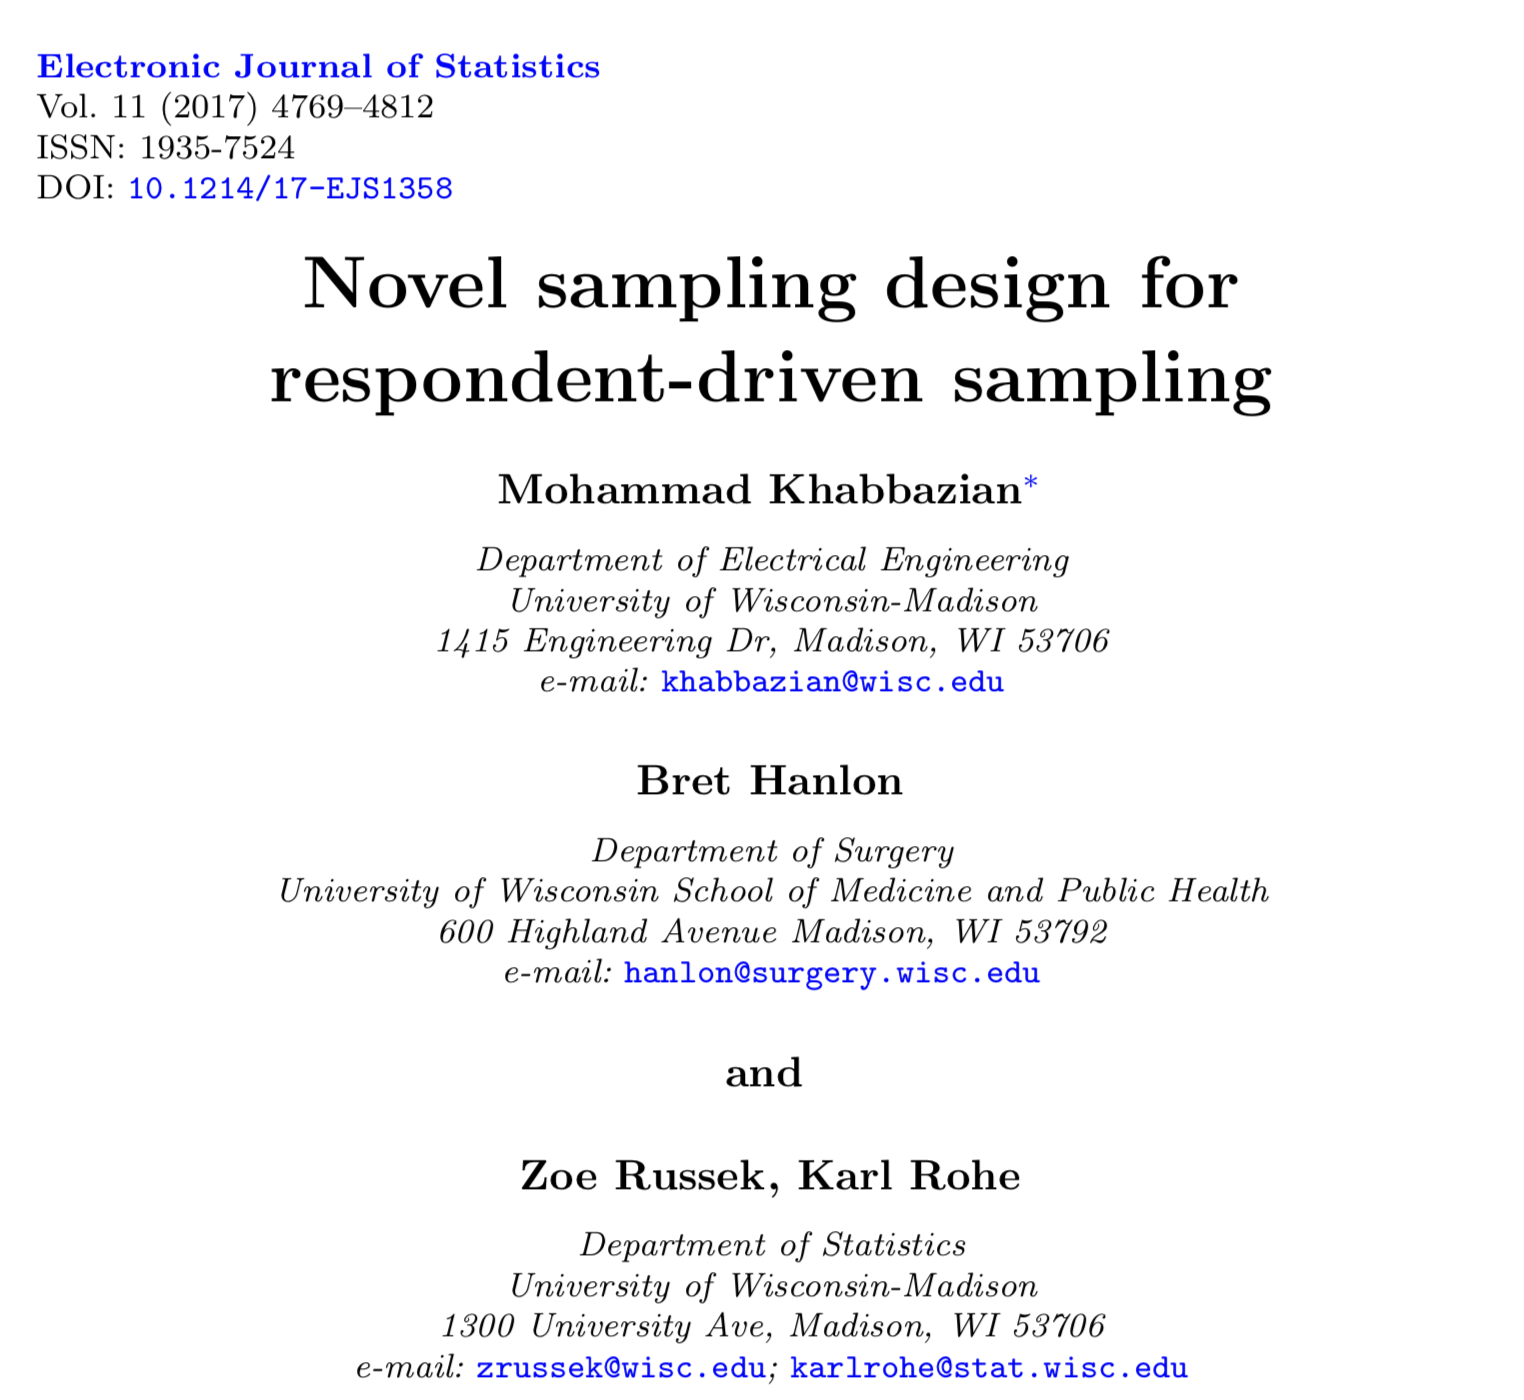
\includegraphics[width=0.6\textwidth]{figures/khabbazian_novel_2017_title}
\end{center}

\vfill
\url{https://doi.org/10.1214/17-EJS1358}
\end{frame}
%%%%%%%%%%%%%%%%%%%%%%%%%%
\frame{
\frametitle{How can we improve RDS? Diagnostics}
Diagnostics that can be run as the sample progress.  In this case, we might actually be able to correct problems during data collection, but this is not without difficulty.

\vfill
Examples from a study of men who have sex with men in Dhaka, Bangladesh (Johnston et al. 2007).  7 seeds grew to a sample size of 531 in 7 weeks.  Thanks to Lisa Johnston for providing the data.
}
%%%%%%%%%%%%%%%%%%%%%%%%%%%%%%%
\frame{
\frametitle{How can we improve RDS? Diagnostics}

Plot the cumulative estimate over time. In this case, the estimate doesn't really stabilize.    
\begin{center}
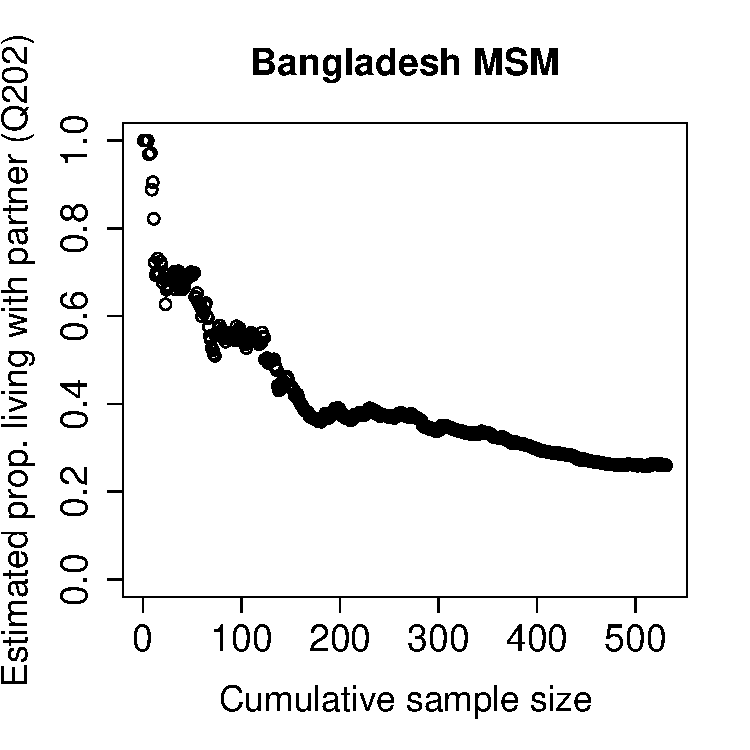
\includegraphics[width=0.5\textwidth]{figures/bang_livingwithpartner_trace_slides}
\end{center}

}
%%%%%%%%%%%%%%%%%%%%%%%%%%%%%%%
\frame{
\frametitle{How can we improve RDS? Diagnostics}

Batched estimates look even worse.
\begin{center}
\includegraphics<1>[width=0.5\textwidth]{figures/bang_livingwithpartner_batchedmeans_slides}
\end{center}

}
%%%%%%%%%%%%%%%%%%%%%%%%%%%%%%%
\frame{
\frametitle{How can we improve RDS?  Diagnostics}
Plot the estimates for each seed separately; inspired by (but different from) $\hat{R}$ method of Gelman and Rubin (1992).
\begin{figure}
  \centering
  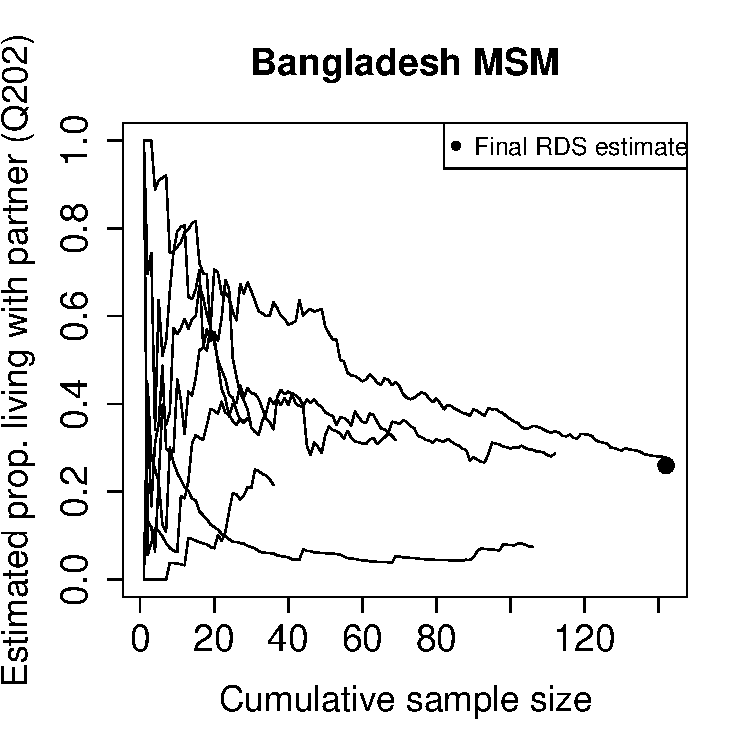
\includegraphics[width=0.5\textwidth]{figures/bang_livingwithpartner_parallelchains_slides}
\end{figure}
}
%%%%%%%%%%%%%%%%%%%%%%%%%%%%%%%
\frame{
\frametitle{How can we improve RDS?}
Look for burn-out as sample progresses.  The degree of respondents decreases over time as the sample progresses.
\begin{figure}
  \centering
  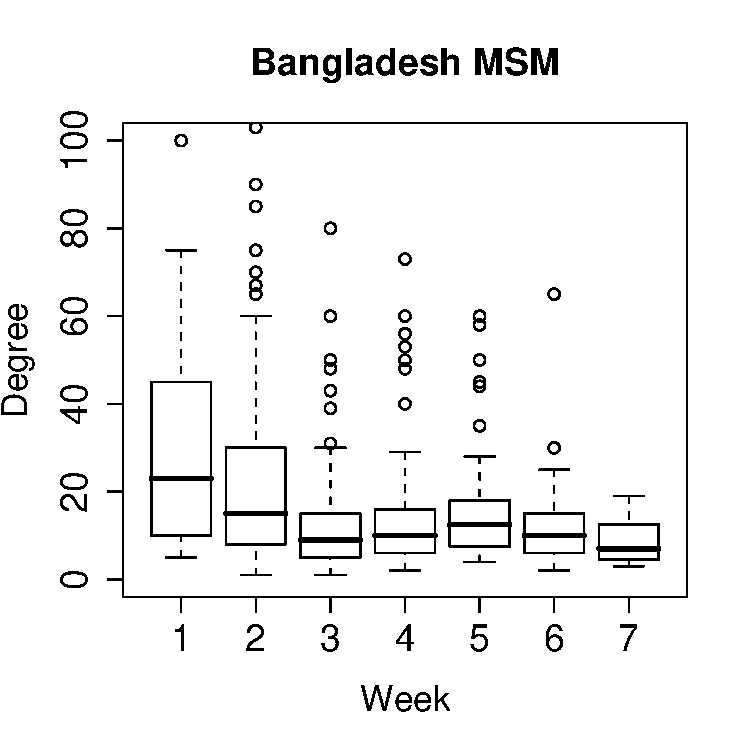
\includegraphics[width=0.5\textwidth]{figures/bang_boxdegree_week_slides}
\end{figure}
}
%%%%%%%%%%%%%%%%%%%%%%%%%%%%%%%
\begin{frame}

\begin{center}
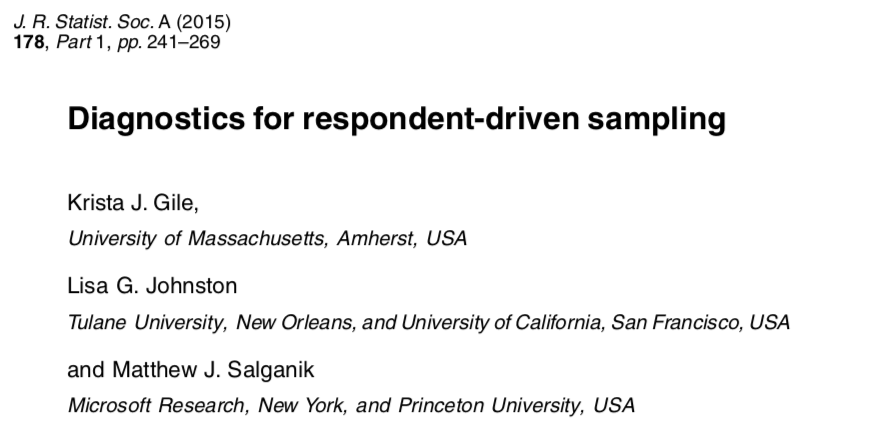
\includegraphics[width=0.6\textwidth]{figures/gile_diagnostics_2015_title}
\end{center}

\vfill
\url{https://doi.org/10.1111/rssa.12059}

\end{frame}
%%%%%%%%%%%%%%%%%%%%%%%%%%%%%%
\begin{frame}
\frametitle{Where are we and where are we going?}

\begin{center}
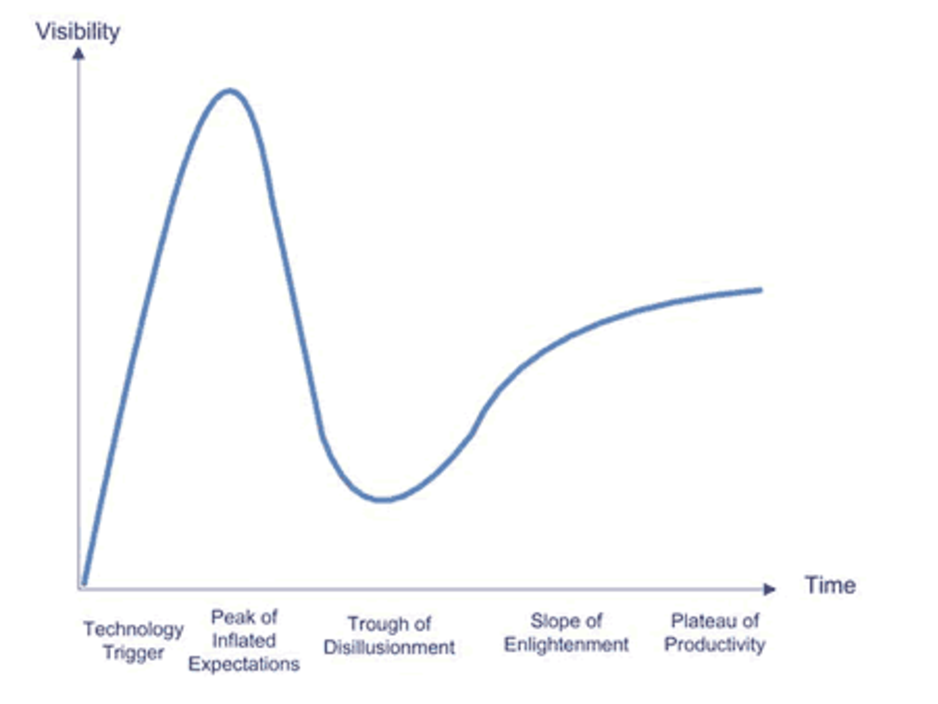
\includegraphics[width=0.6\textwidth]{figures/hype_cycle}
\end{center}

\vfill
Gartner consulting.
\end{frame}
%%%%%%%%%%%%%%%%%%%%%%%
\frame{
\frametitle{Conclusion}

\begin{itemize}
\item Network-based sampling methods can help us collect data from hidden populations, such as the groups most at-risk for HIV.
\pause
\item Under certain conditions, people are selected with probability proportional to degree.
\pause
\item If people are selected with probability proportional to degree, then it is possible to produce estimates that are unbiased (correct on average).
\pause
\item Even if all the conditions are met, respondent-driven sampling seems to have high sample-to-sample variability because of the properties of real social networks (specifically bottlenecks between groups that have differnt characteristics).
\end{itemize}

}
%%%%%%%%%%%%%%%%%%%%%%%%%%%%%%%
\frame{

Next class:
\begin{itemize}
\item Granovetter, M. (1973). ``The strength of weak ties.'' \textit{American Journal of Sociology}.
\item Smith, S. (2005). ``"Don't put my name on it": Social capital activation and job-finding assistance among the black urban poor.'' \textit{American Journal of Sociology}.
\end{itemize}

}
%%%%%%%%%%%%%%%%%%%%%%%%%%%%%%%

\end{document}
